\chapter{Resultados}
\label{c.resultados}

\section{Performance dos Classificadores}

As tabelas e gráficos a seguir mostram os resultados que foram obtidos na fase de Desenvolvimento. Nas tabelas \ref{r.t1} e \ref{r.t2}, constam os números de características e os valores de acurácia obtidos pelos classificadores ótimos encontrados tanto na abordagem de força bruta quanto na abordagem do RFE, respectivamente. Depois, são apresentados os gráficos \ref{r.graf1} e \ref{r.graf2} que ilustram as diferenças de valores entre esses dados para as duas abordagens.



\begin{table}[h!]
  \begin{center}
    \caption{Resultados da abordagem de Força Bruta}
    \label{r.t1}
    \begin{tabular}{l|c|c} % <-- Alignments: 1st column left, 2nd middle and 3rd right, with vertical lines in between
      \textbf{Classificadores} & \textbf{Acurácia} & \textbf{Nº de Características}\\
      \hline
      Árvores de Decisão & 0.996604 & 6\\
      Florestas Aleatórias & 0.997910 & 5\\
      AdaBoost & 0.993208 & 9\\
      NB Multinomial & 0.894723 & 4\\
      NB Bernoulli & 0.840125 & 10\\
      SVC Linear & 0.958986 & 5\\
    \end{tabular}
  \end{center}
\end{table}

\begin{table}[h!]
  \begin{center}
    \caption{Resultados da abordagem utilizando RFE}
    \label{r.t2}
    \begin{tabular}{l|c|c} % <-- Alignments: 1st column left, 2nd middle and 3rd right, with vertical lines in between
      \textbf{Classificadores} & \textbf{Acurácia} & \textbf{Nº de Características}\\
      \hline
      Árvores de Decisão & 0.994775 & 7\\
      Florestas Aleatórias & 0.995559 & 39\\
      AdaBoost & 0.996342 & 16\\
      NB Multinomial & 0.950365 & 17\\
      NB Bernoulli & 0.869905 & 10\\
      SVC Linear & 0.956374 & 12\\
    \end{tabular}
  \end{center}
\end{table}

\begin{figure}[h]
\caption{Comparativo de Acurácias.}
\centering
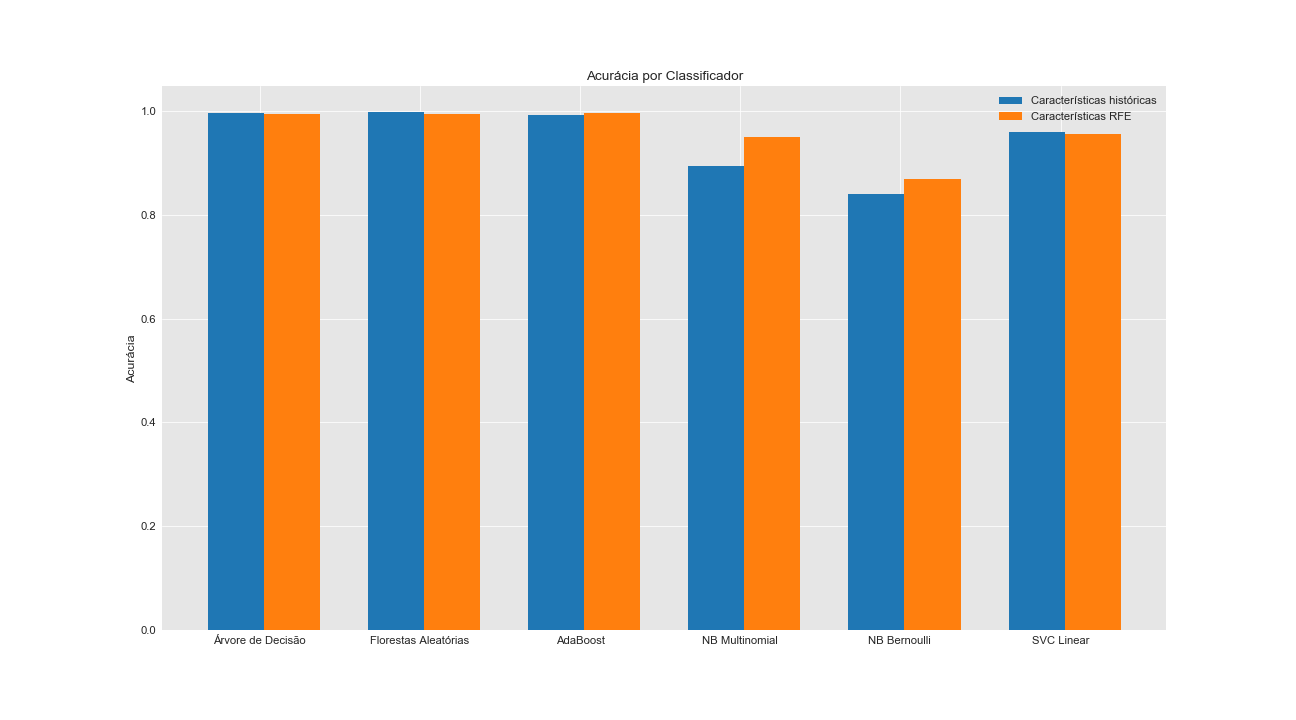
\includegraphics[scale=0.30]{figs/ComparativoAcuracias.png}
\label{r.graf1}
\legend{\small Fonte: Elaborada pelo autor.}
\end{figure}

\begin{figure}[h]
\caption{Comparativo de Número de Características.}
\centering
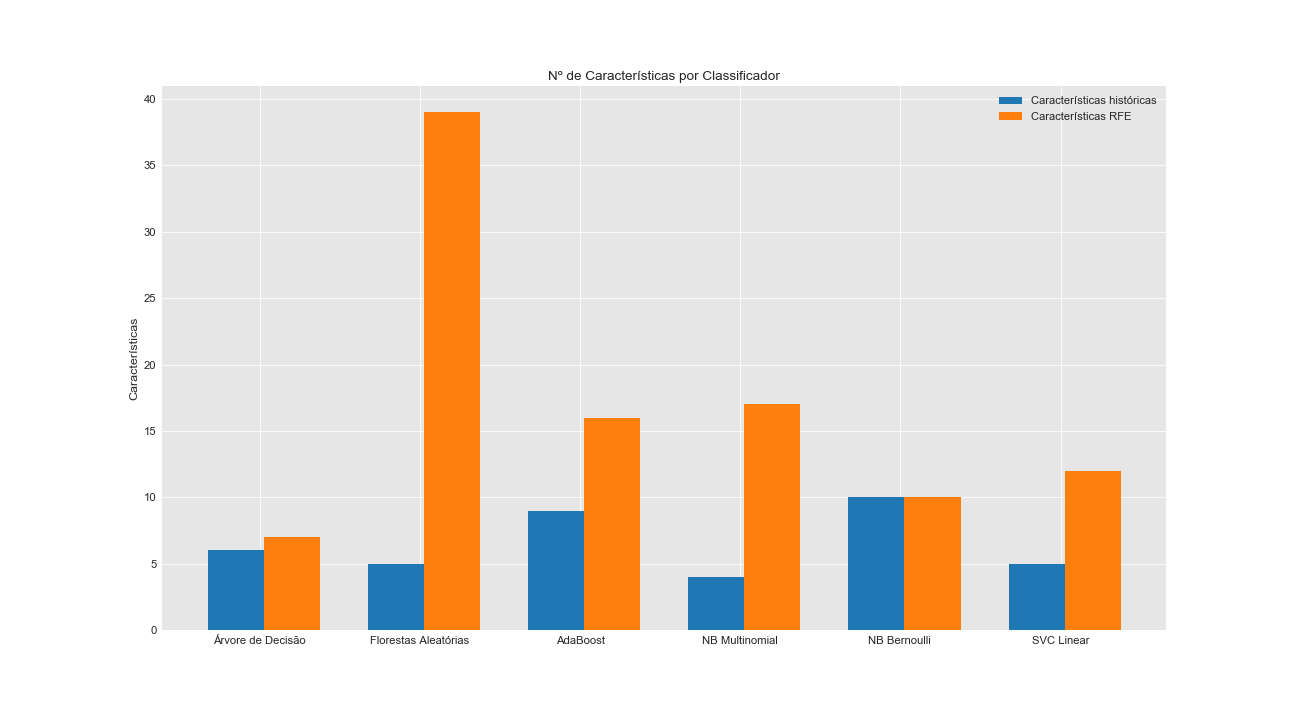
\includegraphics[scale=0.30]{figs/ComparativoCaracs.png}
\label{r.graf2}
\legend{\small Fonte: Elaborada pelo autor.}
\end{figure}

\section{Características}

Esta seção apresentará alguns gráficos que buscam ilustrar a distribuição de características presentes nas duas abordagens. A figura \ref{r.graf3} mostra a quantidade de vezes que uma característica foi utilizada pelos classificadores na abordagem de Força Bruta, enquanto as figuras \ref{r.graf4} e \ref{r.graf5} mostram as dez características que foram mais e menos utilizadas, respectivamente, na abordagem RFE. Por fim, o último gráfico mostra a frequência das características históricas na segunda abordagem de maneira isolada. 

\begin{figure}[h]
\caption{Frequência de Características na abordagem de Força Bruta.}
\centering
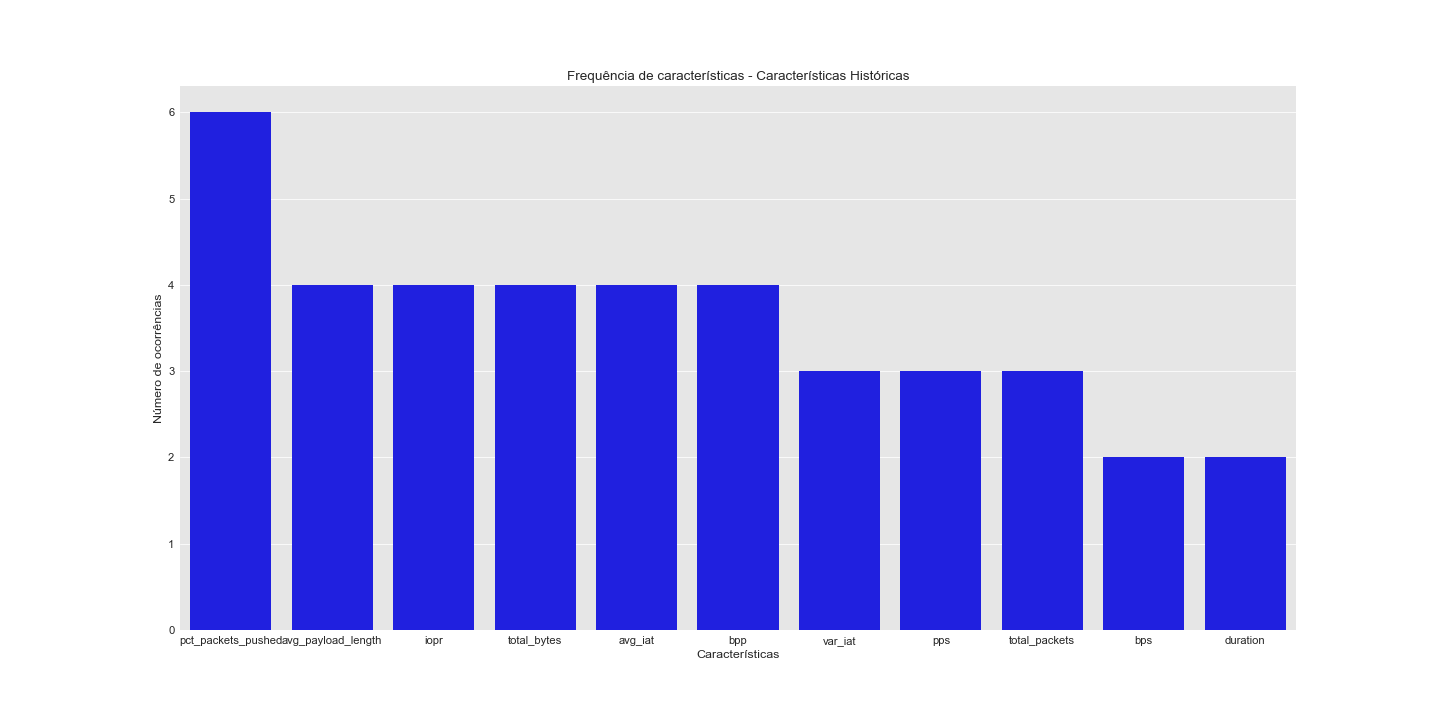
\includegraphics[scale=0.30]{figs/CaracteristicasMetodo1.png}
\label{r.graf3}
\legend{\small Fonte: Elaborada pelo autor.}
\end{figure}

\begin{figure}[h]
\caption{Características mais frequentes na abordagem de RFE.}
\centering
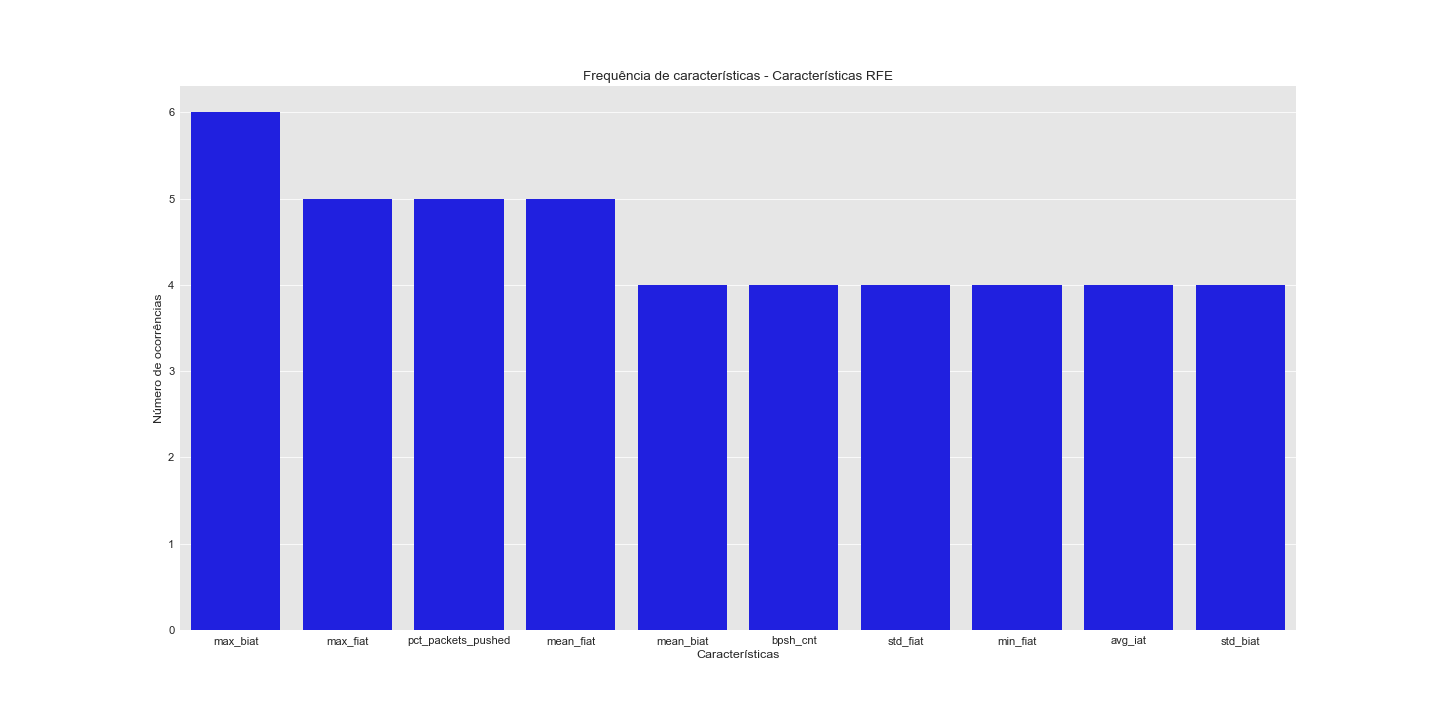
\includegraphics[scale=0.30]{figs/CaracteristicasMetodo2.png}
\label{r.graf4}
\legend{\small Fonte: Elaborada pelo autor.}
\end{figure}

\begin{figure}[h]
\caption{Características menos frequentes na abordagem de RFE.}
\centering
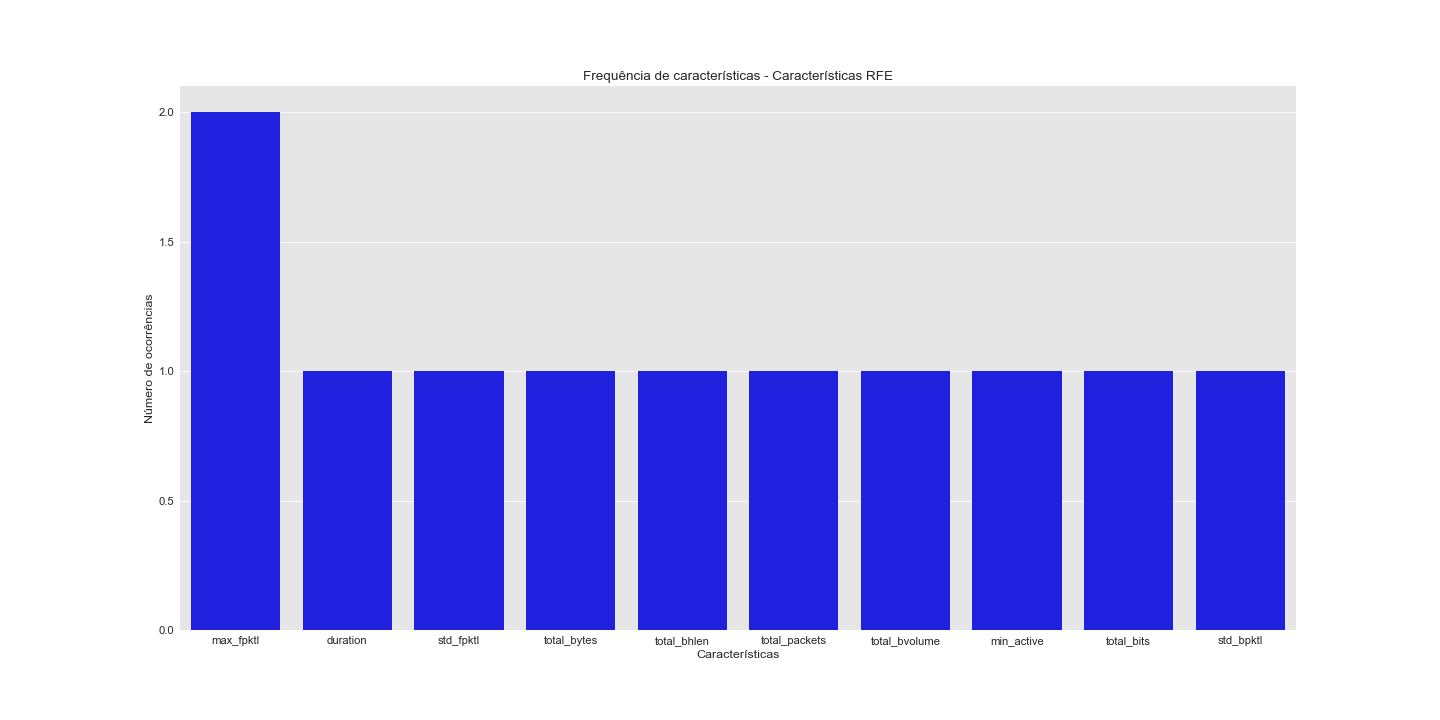
\includegraphics[scale=0.30]{figs/CaracteristicasMetodo2-menos.png}
\label{r.graf5}
\legend{\small Fonte: Elaborada pelo autor.}
\end{figure}

\begin{figure}[h]
\caption{Frequência de Características Históricas na abordagem de RFE.}
\centering
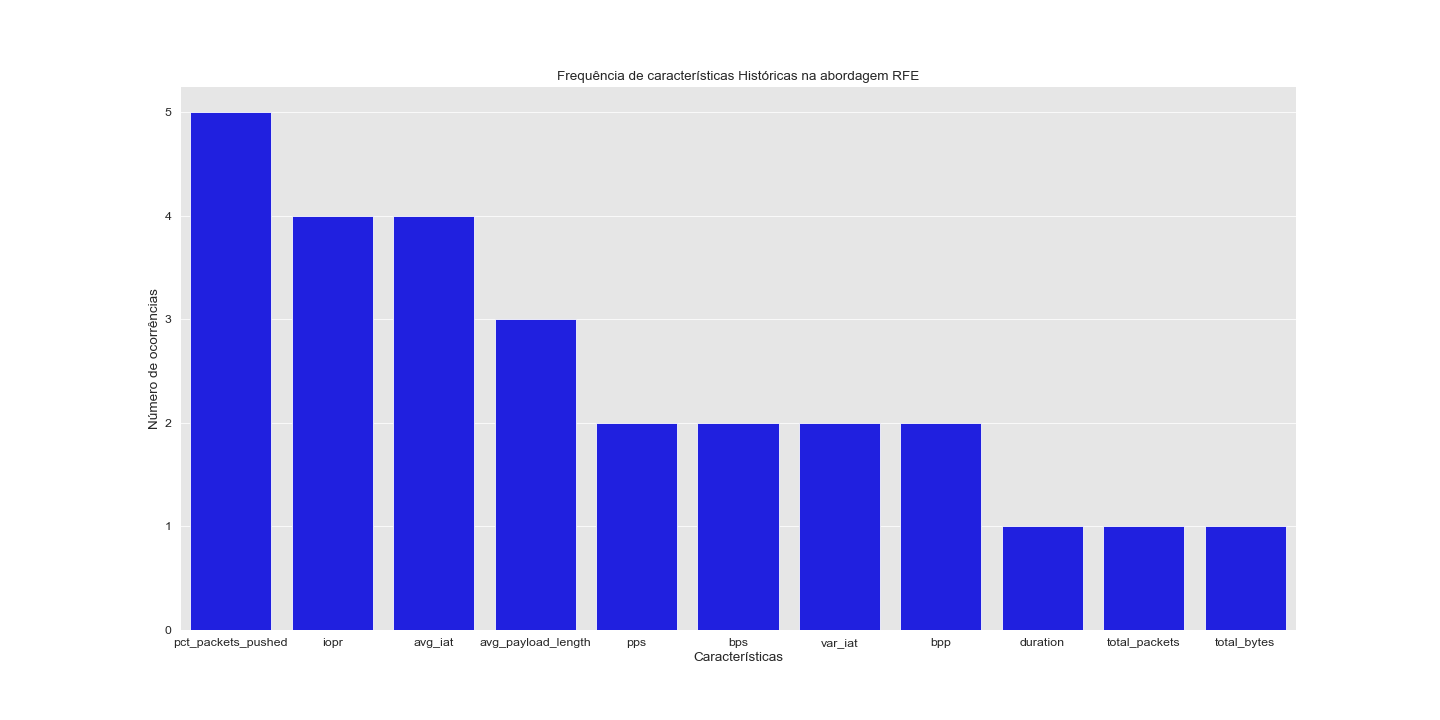
\includegraphics[scale=0.30]{figs/CaracteristicasSVM.png}
\label{r.graf6}
\legend{\small Fonte: Elaborada pelo autor.}
\end{figure}

\section{Hiper-parâmetros}

Esta seção irá apresentar os resultados obtidos pela otimização de Hiper-parâmetros feita para o algoritmo de SVM. A tabela \ref{r.t3} contém os valores de acurácia obtidos para cada Kernel, além dos parâmetros ótimos obtidos no processo. Por fim, a figura \ref{r.grafgrid} apresenta a variação na acurácia para cada Kernel.

\begin{table}[h!]
  \begin{center}
    \caption{Resultados da otimização de Hiper-parâmetros do SVM}
    \label{r.t3}
    \begin{tabular}{l|c|c} % <-- Alignments: 1st column left, 2nd middle and 3rd right, with vertical lines in between
      \textbf{Kernel} & \textbf{Acurácia} & \textbf{Parâmetros}\\
      \hline
      Linear & 0.996604 & C:100\\
      RBF & 0.978840 & C: 100,$\gamma$: 0.001\\
      Sigmoidal & 0.749477 & C: 10,$\gamma$: 0.0001, r:0\\
    \end{tabular}
  \end{center}
\end{table}

\begin{figure}[h]
\caption{Comparativo de Acurácia dos Kernels do SVM.}
\centering
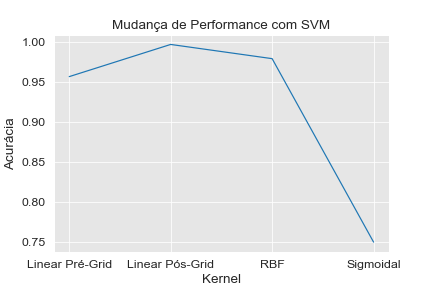
\includegraphics[scale=0.7]{figs/Hiperparametros.png}
\label{r.grafgrid}
\legend{\small Fonte: Elaborada pelo autor.}
\end{figure}